% Results and discussion: the sequential baseline and the measured comparison (issue #67).
% Numbers come from results/phase2/baseline_cycles.csv (#64) and the array's
% results/phase1/cycle_counts.csv, results/phase2/cycle_counts.csv and
% results/phase2/tiled_cycles.csv (#69); the figure from model/perf_model.py (#73).
% Clock frequencies and resources come from results/phase2/synth/synth_summary.csv (#75).

\subsection{Comparison with a Sequential Baseline}
A speed-up means little without a fair reference, so we built the best design that uses a single MAC unit and measured it in the same way as the array. The baseline, \texttt{seq\_matmul}, has exactly the parameters, ports and address map of the accelerator's top level, so the same testbench procedure and the same golden vectors drive both designs, and their results are compared bit for bit.

Inside, the baseline has one multiplier and one adder with the arithmetic of the PE's MAC: the signed 16-bit product is sign-extended to the 32-bit accumulator. It computes $C$ one element at a time in row-major order. Each element takes $k_{\mathrm{len}}$ cycles, one product per cycle, so a run is busy for
\begin{equation}
N^2 k_{\mathrm{len}}
\label{eq:basebusy}
\end{equation}
cycles, 64 for $N = k_{\mathrm{len}} = 4$. There is no clear or capture cycle. The running sum restarts at the first product of each element, from zero in a normal run and from the element's stored value in an accumulate run, and each finished element is written into $C$ in the cycle of its last product. The baseline therefore accumulates across chunks exactly as the array does, and a tiled product runs through it with the same host procedure (Section~III-E). One difference is visible to the host: the baseline overwrites $C$ element by element during a run, so $C$ is valid only from \texttt{done} until the next \texttt{start}, whereas the array keeps the previous $C$ readable until its capture cycle. Matching that would need a second $N \times N$ result store, $16 \times 32 = 512$ flip-flops for $N = 4$, which would inflate the baseline's area in the resource comparison below.

The testbench drove the baseline through every vector set that the accelerator runs: the 106 Phase~1 cases, the 112 $K \neq N$ cases and the 26 tiled products, cut into tiles and accumulate chunks by the same host procedure. It gave the golden $C$ in every case, and every run was busy for exactly $N^2 k_{\mathrm{len}}$ cycles. The captures in \path{results/phase2/waveforms/} show it cycle by cycle: \texttt{seq\_matmul.png} builds one element of $C$ over $k_{\mathrm{len}}$ products, and \texttt{seq\_matmul\_run.png} shows a whole 64-cycle run. With $k_{\mathrm{len}} = N = 4$ that is 64 cycles against 12 for the array, a speed-up of $64 / 12 = 5.3$ in busy cycles. At $k_{\mathrm{len}} = K_{\max} = 16$ it is 256 against 24, a speed-up of 10.7. The array's fill and drain cost $2N$ cycles per run whatever $k_{\mathrm{len}}$ is, while the baseline's time grows by $N^2$ cycles for every extra element of the inner dimension, so the gap widens with the run length.

Table~\ref{tab:speedup} compares the two designs on the directed tiled products. In busy cycles the array is 7.5 to 11.0 times faster on the five directed products with more than one element, and the speed-up grows with the inner dimension $K$: the array pays its fill and drain once per chunk, while the baseline pays $N^2$ cycles for every element of $K$. On the smallest product, $1 \times 1 \times 1$, a single multiply-accumulate, the array's fill and drain dominate and the speed-up is only 1.8. Over all 26 products the busy-cycle speed-up ranges from 1.8 to 11.0.

End to end the picture changes. Both designs load the operands and read the result through the same one-element ports, so those cycles are the same for both, and they dominate the array's total. The total speed-up is 1.2 to 3.5 across the 26 products: 2.7 for the $8 \times 8 \times 8$ product, exactly as Section~III-E predicted, against 8.0 for the busy cycles alone. Fig.~\ref{fig:cycles} shows the same effect for square products up to $64 \times 64 \times 64$: for large products the array's busy time is about an order of magnitude below the baseline's, but its total is set by the ports. A faster host interface would raise the end-to-end speed-up towards the busy-cycle one.

\begin{figure}[t]
\centering
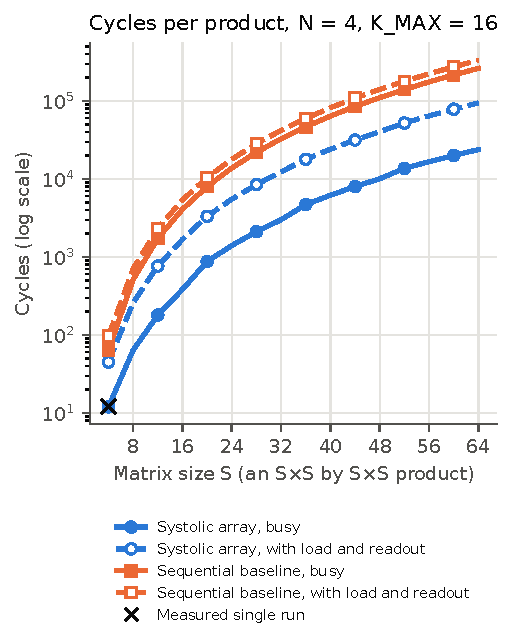
\includegraphics[width=0.85\columnwidth]{cycles_vs_size}
\caption{Cycles of an $S \times S$ by $S \times S$ product on the $4 \times 4$ array and on the baseline, from the cycle model, which matches every measured run and tiled product. Busy cycles are solid, and totals with loading and readout are dashed.}
\label{fig:cycles}
\end{figure}

\textbf{Time and resources.} The two designs also run at different clocks. After place and route on the ECP5 LFE5U-25F, the $4 \times 4$ array reaches 56.83~MHz and the baseline 52.16~MHz, so every cycle speed-up above grows by a factor of 1.09 in time. A run with $k_{\mathrm{len}} = 4$ takes 211~ns on the array and 1227~ns on the baseline, 5.8 times longer, and a run with $k_{\mathrm{len}} = 16$ takes 422~ns against 4908~ns, 11.6 times longer. On the 26 tiled products, with the host ports clocked at each design's own frequency, the busy-time speed-up is 1.9 to 12.0 and the end-to-end speed-up 1.3 to 3.8.

The baseline completes one multiply-accumulate per busy cycle, 52.2 million per second for any $k_{\mathrm{len}}$. The array completes 303 million per second with $k_{\mathrm{len}} = 4$ and 606 million with $k_{\mathrm{len}} = 16$. Per resource, at $k_{\mathrm{len}} = 16$ the array completes 242 thousand per second for each LUT against 14.0 thousand for the baseline, 17 times as many, and 8.2 times as many for each flip-flop, because it uses 2506 LUTs and 2287 flip-flops against the baseline's 3735 and 1617. Per multiplier the baseline is ahead: its single multiplier works in every busy cycle, whereas each of the array's 16 averages 37.9 million per second at $k_{\mathrm{len}} = 16$ and 18.9 million at $k_{\mathrm{len}} = 4$, because a PE waits during the fill and drain. The array's speed therefore comes from its 16 multipliers, not from extra logic.
